\chapter{Background}
In this chapter a selection of terms is explained which gives a basis to understand the rest of this thesis. This background is created with the assumption that the reader has a basic background in Machine Learning and (Convolutional) Neural Networks.


\section{Region of Interest}
The Region of Interest problem is a widely studied problem in which the goal is to estimate the amount of pedestrians given a single image. Directly predicting the count given a Neural Network is a hard task, because of the lack of supervision, this would require a large amount of samples to accurately solve this task. All recent State-of-the-Art methods therefore use an intermediate representation to give the model enough supervision to perform Crowd Counting with a low amount of training samples.

In the early days of Crowd Counting several methods have been proposed which use \emph{detection-based} methods to estimate the amount of pedestrians \cite{Dalal2005, Dollar2012} . Several papers were introduced which tried to detect only the head \cite{Subburaman2012} and others tried to focus on general part detection \cite{Wu2007, Lin2010}. These methods rely on individually detecting the pedestrians. This becomes much harder when occlusion of the pedestrians start to happen. This is why the performance of these methods start to degrade when the density of the pedestrians in an image start to increase.

Later papers introduced a \emph{regression-based} solution, which tries to predict the amount of pedestrians in crowd blobs \cite{Chan2009, Idrees2013, zheng_cross-line_2019}. Using SVM or other regressor methods and several features such as the amount of foregrounds pixels of the blob and detected key points the count inside crowd blobs were predicted. Regression based solutions were an improvement over the detection methods, but still lack the capabilities to estimate pedestrians counts in highly occluded areas.

\subsection{Density Map}

\begin{figure}[h]
\centering
\includegraphics[width=1.0\textwidth]{images/example_count_map}
\caption{Example of generated density map on the right side, for the left image}
\label{fig:density_map}
\end{figure}

With the introduction of Convolutional Neural Networks in the field of Crowd Counting density maps were proposed as well to count pedestrians \cite{Zhang2016, Liu2019, li2018csrnet}. A \emph{density map} (Figure \ref{fig:density_map}) used for Region of Interest is a map which represents the density of pedestrians of each pixel. The density map is generated by taking the locations of each pedestrian ($p=\begin{bmatrix} x_p \\ y_p \end{bmatrix}$ in equation \ref{eq:density_pixel}) and place those locations on the the density map.

Individual dots are very hard for a Neural Network to detect correctly and are proned to errors. To circumvent this a Gaussian shaped circle is created around this location, still with with a sum of 1. The amount of pedestrians in the frame can be extracted from the density map by taking the sum over all the pixels of the density map (Equation \ref{eq:density_sum}, where $D_t(p)$ is the density for location $p=\begin{bmatrix} x_p \\ y_p \end{bmatrix}$ for trainings frame $t$).

\begin{equation}
\label{eq:density_pixel}
	D_t(p) = \frac{1}{2 \pi \sigma_p^2}\sum_{p\in P} e^{\frac{(x_p-x)^2+(y_p-x)^2}{-2 \sigma_p^2}}
\end{equation}

\begin{equation}
	\label{eq:density_sum}
	C_t = \sum_{p\in P} D_t(p)
\end{equation}

Several methods have been presented to optimize the generation of density maps \cite{Zhang2016, li2018csrnet, Wan2019}. For most medium dense frames the difference in methods is minimal. Often in benchmarks with medium dense frames a fixed sigma is used ($\sigma_p=\sigma_i$ in equation \ref{eq:density_pixel}). For highly dense frames the use of different methods can have a difference, especially when the difference in size between close pedestrians and pedestrians in the background is large \cite{li2018csrnet}.
\todo{A bit more papers of recent improvements}

\section{Flow Estimation}
The research which is done on the Flow Estimation problem is widely used. Approaches on this topic can be used in a wide range of applications which makes it very interesting. Already in the early 1980's Horn and Schunck \cite{Horn1981} published the first paper which tried to predict flow. Since then lot's of different approaches have been published \cite{Memin1998, Bruhn2005, Brox2014}. Long conventional mathematical approaches have ruled the flow estimation field. Later also learnable models were introduced \cite{Pock2008, Wedel2009}.

\begin{figure}[h]
\centering
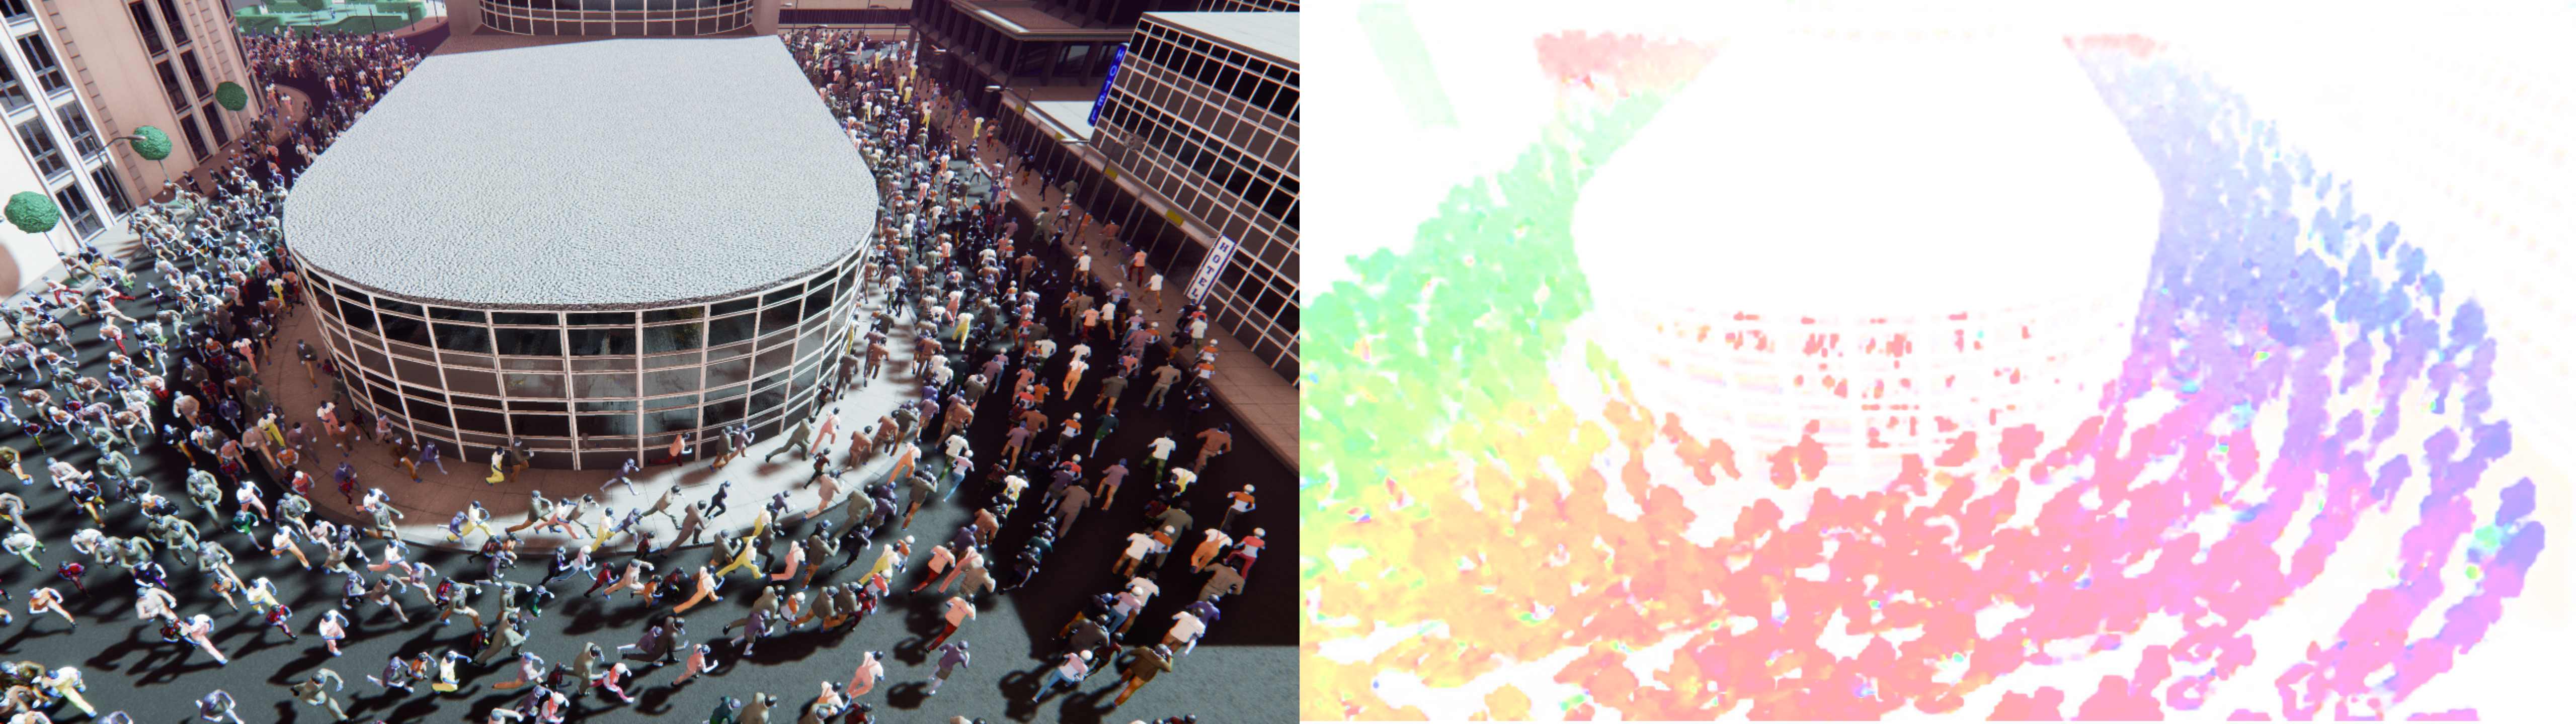
\includegraphics[width=1.0\textwidth]{images/example_flow_map}
\caption{Example of generated velocity map on the right side, for the left image}
\label{fig:flow_map}
\end{figure}


Recent papers however make use of Convolutional Neural Network based models \cite{Dosovitskiy2015, ilg_flownet_2016, sun_pwc-net_2018, Ranjan2017, Hui2018}. These model predict pixel-precise velocity maps. The \emph{velocity map} (Figure \ref{fig:flow_map}) is a map which predict per pixel of the frame the amount of movement to another location. In equation \ref{eq:flow_basis}, $V_t(p)$ shows the velocity map as a difference between the location of the pixel in the current frame ($p$) and the location of this pixel in the next frame ($N_t(p)$).

\begin{equation}
\label{eq:flow_basis}
V_t(p) = N_t(p) - \begin{bmatrix} x_{p} \\ y_{p} \end{bmatrix}
\end{equation}

Creating a real world dataset that utilizes the power of pixel-wise flow estimation is very hard \cite{Dosovitskiy2015}. There are no real world devices which could capture both video and create pixel perfect ground-truths to train the flow estimation models on. Most of the flow estimation benchmarks are therefore generated videos. Computer 3D-engines make it possible to generate pixel-perfect flow estimation based on the generated videos in the engine.

However the large gap in domain and scene between the generated datasets and real world applications \cite{Liu2008}. Recent supervised papers \cite{Dosovitskiy2015, sun_pwc-net_2018} tend to overfit on the datasets. Therefore perform rather poor on real world applications. One solution and promising direction is unsupervised learning \cite{Yu2016, Janai2018, liu_ddflow_2019, liu_selflow_2019}. Early papers only predicted non-occluded pixels \cite{Yu2016, Janai2018}, but recent papers use methods to estimate occluded pixels as well \cite{liu_ddflow_2019, liu_selflow_2019}. Further details about these methods in related work.



\section{Line of Interest}
Line of Interest is very similar to Region of Interest. Where Region of Interest is the interest of the amount of people inside the ROI, the Line of Interest is the focus on the amount of pedestrians that cross the specified line during a certain timeframe. This LOI is defined as a single line between two points $p_1$ and $p_2$.
\todo{Add an image with a line drawn inside the TUB dataset}

With the Line of Interest problem the goal is to give the amount of pedestrians crossing of each side given a set of frames (a pre-captured video or video stream). The output of the prediction should give two numbers $c_1$ and $c_2$ which are the amount of pedestrians crossing from each side.

Only a handful of papers are published about Line of Interest. In the earlier papers \cite{ma_counting_2016, cao_large_2015}, slicing was a widely used approach to estimate the Line of Interest. With slicing a small area, called the LOI area, is taken around the LOI. Over a set of consecutive frames each slice of the frame was taken and stitched together into a single image. On the images slow walking pedestrians appear rather wide and fast walking pedestrians shallow. By counting the amount of pedestrians present on the stitched image, the total amount of pedestrians crossing the line can be counted.

The area is defined by all the pixels that have a maximum distance to the LOI of $d$ and can be projected on the LOI. When projected, the pixels fall between $p_1$ and $p_2$.

Recent papers discard this method \cite{leibe_crossing-line_2016, zheng_cross-line_2019}, because it makes it hard to track pedestrian with different speeds and walking in different directions give artifacts which make it hard to track those pedestrians \cite{leibe_crossing-line_2016}. The slicing method is replaced with an actual frame by frame prediction method. Using two consecutive frames the amount of pedestrians crossing the line is measured. These newer methods predict both location and direction of the pedestrian. 

Based on these new papers, the problem of Line of Interest is divided into three separate problems. Locating the pedestrians (Region of Interest), estimate the direction (Flow Estimation) of the pedestrians and combining these two streams of information into the count for Line of Interest. Further details of this approach will be provided in related work.